The recognition of an object in a scene with precision can be a trick problem to be solved, and to increase the experience with some virtual artifacts calls for a high level of localization accuracy.

This paper presents an approach based a pre-known 3d representation of the scene.

The real time reconstruction of the scene are fundamental to reduce the cumulative error added to the recognition added after each frame because of interest point recognition hardness caused by light variation, textures and other issues studied in this essay.
As proposed in \cite{ISMAR2012}

\begin{figure}[ht!]
\centering
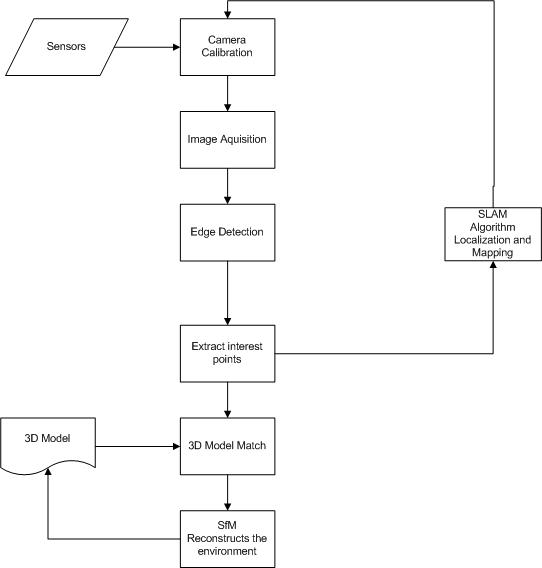
\includegraphics[width=90mm]{images/algorithm.jpg}
\caption{Algorithm Diagram}
\label{algorithm}
\end{figure}


O caminho feliz é ditado por aquisição de imagem, reconhecimento de bordas, reconhecimento de pontos de interesse, model match reconhecimento de 



\subsection{AR Common Flaws}

Jitter
Occlusion

\subsection{Camera Calibration}

\subsubsection{Error Reduction Approach}

Todo frame com a movimentação da camera ou do objeto o rastreamento descasa um pouco, prejudicando a precisão.
Dois métodos são utilizados para reduzir o erro de rastreamento
SLAM utilizado para conferir uma calibracao boa recuperando informacoes de movimento e tentando inferir a posicao da camera


Tenho que ver como vou medir o erro a cada frame, se vai ser um minimo quadrados de pontos importantes com o modelo ou algo mais robusto


\subsection{Image Acquisition}

Etapa simples, tenho que definir qual a latencia de aquisicao de imagens que terei uma quantidade de informacoes suficiente, aqui cabe colocar uma variável para calcular o erro final

\subsection{Edge Detection}

Obter as bordas para depois conseguir retirar os pontos de interesse, aqui cabem filtros ou reconhecedores de padrao.

Também é outra fonte de erro adicionada ao final do modelo.

\cite{Drummond99real-timetracking}


\subsection{Extract Interest Points}

Dependendo do reconhecedor de padrão conseguirei retirar um tipo de ponto de interesse diferente.

Aqui terei uma miriade de reconhecedores que podem adicionar erros ou incertezas ao modelo

\subsection{Model Match}


Eu acho que é a parte que vai mais dar trabalho porque eu vou ter que provavelmente estimar pose para definir projecoes diferentes

\subsubsection{Choosing the apropriate approach to 3d track}



\subsubsection{Real Time Model Reconstruction}

Quando reconhecermos e 


\subsubsection{SLAM}

